\section{Tests realisés pour valider le fonctionnement du TP}
\bframe{
    Les tests réalisés ont simplement été d'ouvrire 2 instances du programme dans 2 sessions de shells différents puis de placer des locks à différents à droit endroit avec le premier et de tester s'ils existent et sont bien reconnus avec le 2e. i.e. :
    \begin{figure}[H]
    \centering
    \hspace{-0.45cm}    
    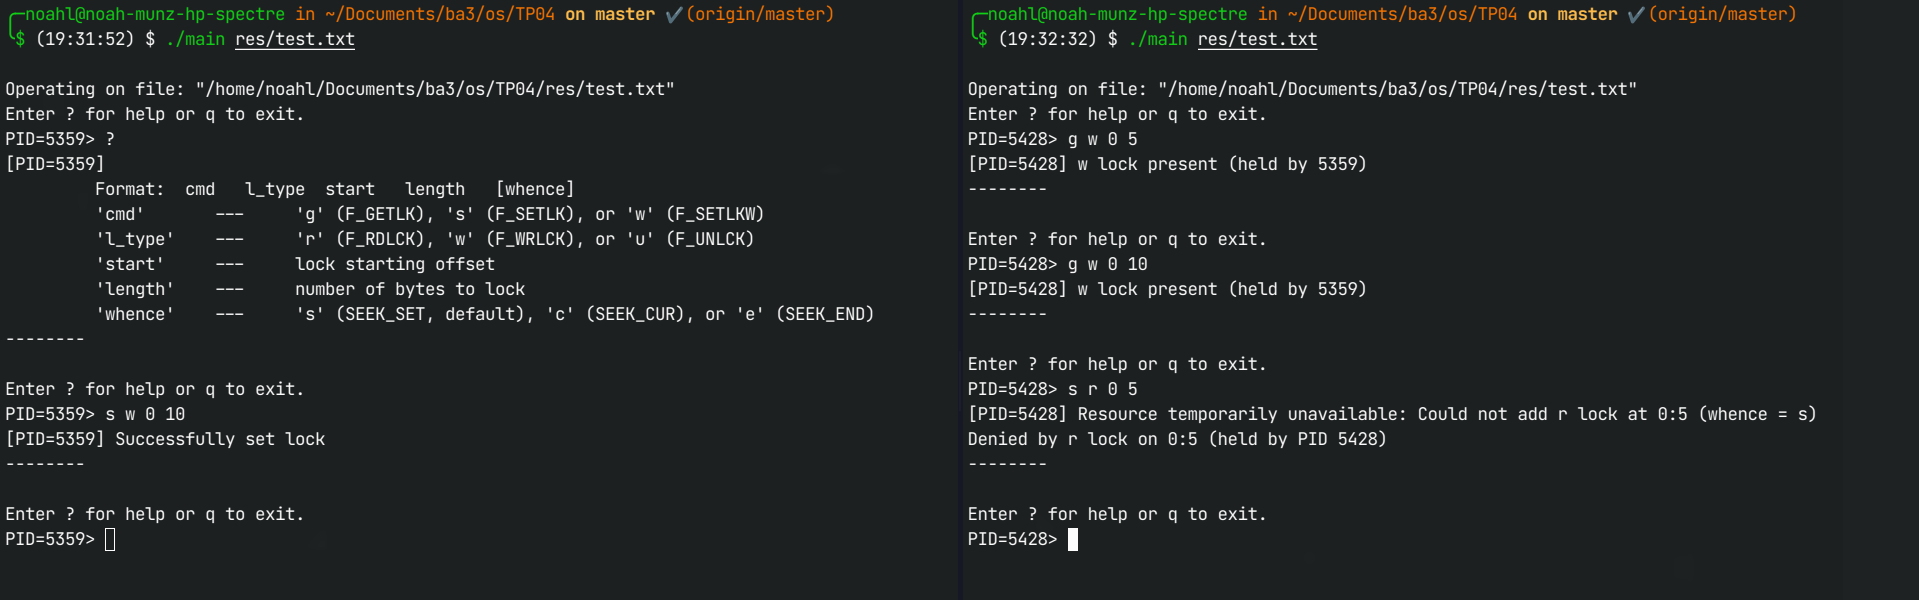
\includegraphics[width=1.03\linewidth,height=5cm]{images/4.tests.png}
    \caption{Test de l'implémentation du TP04.\label{fig:Figure1}}
    \end{figure}
    \unskip
}
